\documentclass[]{beamer}
% \documentclass[handout]{beamer}

\usepackage{caption}
\captionsetup[figure]{labelformat=empty}  % no figure numbers

\mode<presentation>
{
  \usetheme{Warsaw}
  \usecolortheme{default}
  \usefonttheme{default}
  \setbeamertemplate{navigation symbols}{}
  \setbeamertemplate{caption}[]
  \setbeamertemplate{footline}{}
}

% ------------------------------------------------------------------------------
% PACKAGES
% ------------------------------------------------------------------------------
\usepackage{microtype,
			cleveref,
			graphicx,  % graphics library
			url,  % url formatting
			}
\usepackage[T1]{fontenc} % Use EC fonts
\usepackage[utf8]{inputenc}	% Encoding
\usepackage{csquotes}  % manage quotes, inputenc to be loaded first
\usepackage[authoryear]{natbib}  % bibliography
\PassOptionsToPackage{obeyspaces}{url}  % to allow spaces in urls
\PassOptionsToPackage{hyphens}{url}  % to stop urls running off into the side of the page
\usepackage{hyperref}  % cross referencing
\usepackage{cleveref}  %  intelligent cross referencing
\hypersetup{
	colorlinks,
	linkcolor={red!50!black},
	citecolor={blue!50!black},
	urlcolor={blue!80!black}
}

% create a source link
\newcommand<>{\credit}[1]{\par\hfill \tiny \itshape \href{#1}{Source}}

% Turn this on to show toc before each section
%\AtBeginSection[]
%{
%	\begin{frame}<beamer>
%		\frametitle{Plan}
%		\tableofcontents[currentsection]
%	\end{frame}
%}

% ------------------------------------------------------------------------------
% Templates
% ------------------------------------------------------------------------------
%\begin{columns}[T]
%	\begin{column}{.5\textwidth}
%	\end{column}
%	\begin{column}{.5\textwidth}
%	\end{column}
%\end{columns}

% ------------------------------------------------------------------------------
% REFERENCING PACKAGE
% ------------------------------------------------------------------------------
\begin{filecontents}{references.bib}
@misc{pypl,
title = {PopularitY of Programming Language},
author = {Pierre Carbonnelle},
year = 2016,
howpublished = {\url{http://pypl.github.io/PYPL.html}},
organization = {PYPL},
}
@misc{python,
title = {Python},
author = {python},
howpublished = {\url{python.org}},
organization = {Python},
}
@misc{treehouse,
title = {Treehouse},
author = {Treehouse},
howpublished = {\url{https://teamtreehouse.com/}},
}
\end{filecontents}

\title[Python - A shot of inspiration]{Python – A shot of inspiration for day
to day analysis}
\author{Vipin Ajayakumar}
% \institute{}
\date{\today}

\begin{document}
\bibliographystyle{plainnat}

\begin{frame}
  \titlepage
\end{frame}

\begin{frame}{Contents}
  \tableofcontents
\end{frame}

% ==============================================================================
\section{Introduction}
% ------------------------------------------------------------------------------
  \begin{frame}{My programming background}
    \begin{itemize}[<+->]
      \item Comp Sci at A-levels (fundamentals, intro to Visual Basic)
      \item Aerospace engineering degree (not taught much comp sci)
      \item Used VBA in an internship to automate a data entry task
      \item Used Matlab for thesis to model lift with discrete
      vortices
      \item Self-taught Python in final attachment of grad scheme to
      automate a data analysis task
      \item Currently, using Python for day to day tasks and for improvements
      \item Learning JavaScript, \LaTeX, Python, Machine Learning etc. at home
      \item In summary, barely scratched the surface, but I can share the
      little I know. :)
      \item If I can code, then surely you can do it even better!
    \end{itemize}
  \end{frame}

\section{Why bother?}
% ------------------------------------------------------------------------------
  \begin{frame}{Why code rather than use MS Excel?}
    \begin{columns}[T]
      \begin{column}{.5\textwidth}
        \begin{itemize}[<+->]
          \item Increasing complexity of analyses
          \item Spreadsheets cannot cope
          \item Save time
          \item Code exposes logic, a spreadsheet exposes the data
          \item Reduce human error
          \item Improve capability
          \item Enable continuous abstraction
          \item Focus on the more important tasks
        \end{itemize}
      \end{column}
      \begin{column}{.5\textwidth}
        \begin{figure}
          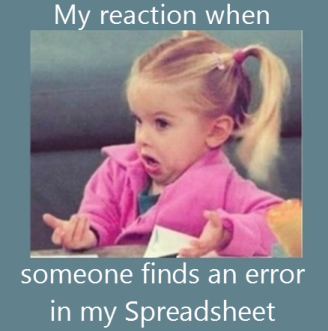
\includegraphics[width=\linewidth,
                           height=\textheight,
                           keepaspectratio]{images/excel.png}
          \credit{http://datapigtechnologies.com/blog/wp-content/uploads/2014/04/041714_0620_ExcelMemeCo27.png}
        \end{figure}
      \end{column}
    \end{columns}
  \end{frame}

  \begin{frame}{What is Python?}
  Courtesy of Wikipedia:
    \begin{itemize}
      \item Python is a programming language
      \item Created by Guido van Rossum in 1991
      \item Two relevant versions: Python 2.7 and Python 3.x
      \item Python 2.x will not be developed much more
    \end{itemize}
  \end{frame}

  \begin{frame}{Why Python?}
    \begin{itemize}
   \item Python is very popular and still gaining in popularity.
      \item Therefore, it has a very active and supportive community.
    \end{itemize}
    \begin{figure}
      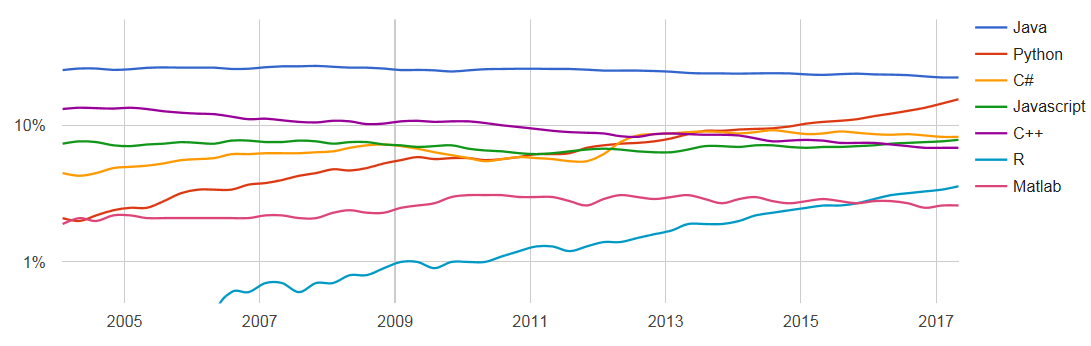
\includegraphics[width=\linewidth,
                      height=0.7\textheight,
                      keepaspectratio]
                      {images/pypl.png}
      \caption{PopularitY of Programming Language \citep{pypl}}
    \end{figure}
  \end{frame}

  \begin{frame}{Why Python?}
    \begin{columns}[T]
      \begin{column}{.5\textwidth}
        \begin{itemize}[<+->]
          \item Beginner friendly
          \item Beautiful syntax
          \item Dynamically typed
          \item Object Oriented
          \item Interpreted
          \item Machine learning support
          \item Cross platform
          \item Open Source
          \item Large and active Stack Overflow community
        \end{itemize}
      \end{column}
      \begin{column}{.5\textwidth}
        \begin{figure}
          
\includegraphics[width=\linewidth,
                          height=\textheight,
                          keepaspectratio]{images/python.png}
          \credit{python.org}
        \end{figure}
      \end{column}
    \end{columns}
  \end{frame}

\section{Learn Python}
% ------------------------------------------------------------------------------
  \begin{frame}{Learning resources}
    \begin{columns}[T]
      \begin{column}{.5\textwidth}
        \begin{enumerate}[<+->]
          \item \href{https://teamtreehouse.com/}{Treehouse} - Python course
          \item \href{https://ocw.mit.edu/courses/electrical-engineering-and-
          computer-science/6-0001-introduction-to-computer-science-and-
          programming-in-python-fall-2016/}
          {Intro to Comp Sci ... in Python
          at MIT}
          \item \href{https://cs50.harvard.edu/}{Harvard CS50 course}
          \item \href{http://amzn.eu/5L0UoHp }{Clean Code} - An essential book on good practice
          \item \href{http://amzn.eu/7B7eB83 }{Python for data analysis} - A good reference book
          \item \href{https://stackoverflow.com/}{Stack Overflow} - Q\&A site
          \item \href{https://www.youtube.com/user/sentdex}{sentdex} or other YouTube channels
          \item \href{https://www.udemy.com/}{Udemy} - Online courses
        \end{enumerate}
      \end{column}
      \begin{column}{.5\textwidth}
        \begin{figure}
          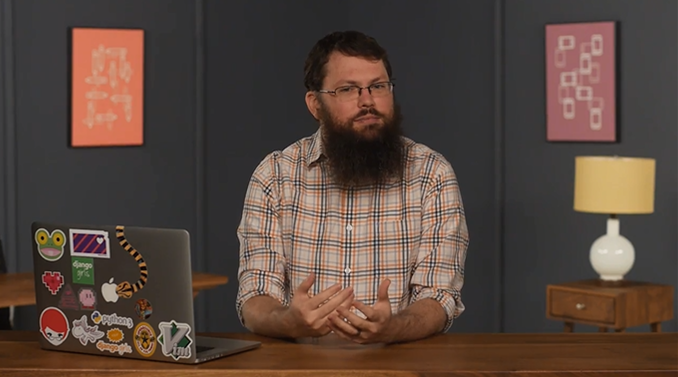
\includegraphics[width=\linewidth,
                          height=\textheight,
                          keepaspectratio]{images/treehouse.png}
          \caption{Python course \citep{treehouse}}
        \end{figure}
      \end{column}
    \end{columns}
  \end{frame}

\section{Apply Python}
% ------------------------------------------------------------------------------
  \begin{frame}{Recommended packages and tools}
  Python packages:
    \begin{itemize}[<+->]
      \item \href{https://docs.python.org/2/library/os.html}{os} provides
      operating system interfaces
      \item \href{https://docs.python.org/2/library/re.html}{re} provides
      expression matching operations
      \item \href{http://pandas.pydata.org/}{pandas} is a powerful data analysis
      library that provides the DataFrame object
      \item \href{http://www.numpy.org/}{numpy} provides a powerful
      N-dimensional array object
      \item \href{http://matplotlib.org/api/pyplot_api.html}{matplotlib.pyplot}
      provides a matlab like plotting framework
    \end{itemize}
  Tools:
      \begin{itemize}[<+->]
      \item PyCharm or Visual Studio Code for editing
      \item git for version control
      \item MS Visio to create diagrams to aid Systems Engineering
    \end{itemize}
  \end{frame}

  \begin{frame}{Typical data analysis procedure}
    \begin{enumerate}[<+->]
      \item Parse a text file
      \item Manipulate the data
      \item Display graphs
    \end{enumerate}
  \end{frame}

\section{Conclusion}
% ------------------------------------------------------------------------------
  \begin{frame}{Weaknesses to be aware of}
    \begin{itemize}[<+->]
      \item Slower processing than lower level languages
      \item Parallelisation possible but not native and not easy
      \item Backward compatibility not guaranteed
    \end{itemize}
  \end{frame}


  \begin{frame}{Conclusion}
    \begin{itemize}[<+->]
      \item There is a strong case for learning and using Python
      \item Links provided to various Python learning resources
      \item A number of key packages can make typical data analysis tasks very
      easy
      \item Potential to expand beyond `just data analysis' to more powerful
      Machine Learning applications
      \item If you need help, please feel free to get in touch!
    \end{itemize}
  \end{frame}

% ------------------------------------------------------------------------------
\begin{frame}{References}
  \bibliography{references}
\end{frame}

\end{document}